\section{Raytracing}
We will now discuss the implemenation of the raytracer used in the system to find the intersection points and shading specular
surfaces. Multiple raytracing threads are created, these threads are passed a pointer to a queue that when read returns a
pixel coordinate that the thread will trace, this queue is written by an additional thread that will write each pixel in the
output image as space becomes available in the queue, the queue is of sufficient size so as the raytracing threads do not
exhaust the thread. In order to signal to the raytracing thread that the render has finished a flag can be set with the pixel
data that indicates that the thread should finish executing one finish signal is sent to each of the threads.

\begin{algorithm}
\begin{algorithmic}
\caption{Raytracing Main Thread}
\For{ 0 to num\_threads}
	\State \Call{start\_thread}{input\_queue, output\_queue}
\EndFor

\For{ 0 to num\_pixels}
	\State pixel\_data $\gets$ \Call{queue\_read}{output\_queue}
	\State \Call{update\_pixel}{pixel\_data}
\EndFor

\end{algorithmic}
\end{algorithm}

\begin{algorithm}
\begin{algorithmic}
\caption{Raytracing Processing Thread}

\State pixel\_data  $\gets$ \Call{queue\_read}{input\_queue}

\While{pixel\_data.continue}
	\State colour $\gets$ black
	\For{each sample in pixel}
		\State colour += \Call{trace\_pixel}{}
	\EndFor
	\State \Call{queue\_write}{output\_queue, pixel\_data.x, pixel\_data.y, colour}
	\State pixel\_data  $\gets$ \Call{queue\_read}{input\_queue}
\EndWhile

\end{algorithmic}
\end{algorithm}

\subsection{Multisampling}
For each pixel that a raytrace thread receives mulitple rays are traced through the scene in order to perform multisampling
on the pixel, this allows us to remove aliasing in the final image and perform districution raytracing, we perform stratified
sampling of the pixel area to calcualte the location of each of the sub-pixels.

\begin{figure}[h]
\centering
\begin{subfigure}[b]{0.4\textwidth}
	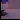
\includegraphics[width=\textwidth]{./images/renders/no-aa.png}
	\caption{1 sample per pixel}
\end{subfigure}
\begin{subfigure}[b]{0.4\textwidth}
	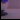
\includegraphics[width=\textwidth]{./images/renders/aa.png}
	\caption{25 samples per pixel}
\end{subfigure}
\end{figure}

\subsection{Scene Traversal}
Each ray that is traced in the scene requires that we traverse the scene in order to find the closest intersection, in
this system we store the objects as a list of pointers to there respective data, as a result of this the scene traversal
algorithm is quite simple, we interate over each of the objects and test if the ray intersects, if not then we continue, if
so we check the intesection $t$ parameter with that of the closest intersection found up to that point
(initially set to $\infty$). If an intersection is found we then call the shade function of the intersecting objects in
order to find the radiance value for this ray, otherwise we set the colour to a default sky colour found in the scene
description.

\begin{algorithm}
\begin{algorithmic}
\caption{Scene Traversal Algorithm}
\State colour   $\gets$ scene.sky\_colour
\State record.t $\gets \infty$
\For{object $\in$ scene}
	\State new\_record $\gets$ \Call{intersects}{ray, object}
	\If{new\_record.hit \textbf{and} new\_record.t $\textless$ record.t}
	\State record $\gets$ new\_record
	\EndIf
\EndFor
\If{record.hit}
	\State colour $\gets$ \Call{shade}{scene, record}
\EndIf
\State \Return colour
\end{algorithmic}
\end{algorithm}

\subsubsection{Self Intersection}
Due to the floating point errors in the calculation of intersection tests the point of intersection that is reported may be
slightly incorrect, this inaccuracy can cause issues for reflection, transmission and shadows as the intersection of the
specular or shadow ray reports an intersection point close to the original intersection point, this can cause artifacts in
the final render, to remedy this issue we use a small offset in the direction of the incident ray so that the origin of the
new ray is slightly above the intersection point.

\subsubsection{Volume Intersection}
Unlike intersection with all other object types the intersection with a participating media is non deterministic as the
media represents a stochastic distribution of particals as a result an intersection test with the same ray may return
a different intersection point if performed multiple times, this property allows us to perform multiple samples that
will converge to the correct appearence of the participating media allowing affects such as objects embedded within
the media to be visible but occluded by the media.

\subsubsection{Intersection Records}
Each intersection that is performed in the system gathers certain data that is needed by later stages of the system, for
example an intersection with a triangle will not only return the $t$ parameter for the intersecting ray but also
barycentric coordinates that can be used to interpolate properties of the triangle vertices across the surface of the
triangle. In order to store this information a pointer to a intersection records is passed as a parameter for each
intersection test, this intersection record is then used during the shading section of the raytracing algorithm.


\newpage
\section{Shading}
Once we have found a point of intersection we must now calculate the colour at that point, this will take into account the
reflecance properties of the object and the photon map surrounding it, this will in effect be an evaulation of the rendering
equation, which we will evaluate by spliting the equation into several components, these components are direct illumination,
specular reflection and transmission which we evaluate using raytracing and diffuse interreflection and caustcs which will
use the photon map to estimate the radiance.

Recall from Chapter~\ref{chap:lit}  the rendering equation is given in terms of incoming and outcoming radiance, omitting
emitted radiance we can rewrite the rendering equation with each of the components seperated \cite{JensenBook}

\begin{align*}
L_{r}(x, \omega) =&
			\int_{\Omega}
				f_{r}(x, \omega, \omega')
				L_{i,l}(x,\omega,\omega')
				(\omega \cdot n)d\omega'
			+\\
		&	\int_{\Omega}
				f_{r,S}(x, \omega, \omega')
				(
				L_{i,d}(x,\omega,\omega')
				+
				L_{i,c}(x,\omega,\omega')
				)
				(\omega \cdot n)d\omega'
			+\\
		&	\int_{\Omega}
				f_{r,D}(x, \omega, \omega')
				L_{i,c}(x,\omega,\omega')
				(\omega \cdot n)d\omega'
			+\\
		&	\int_{\Omega}
				f_{r,D}(x, \omega, \omega')
				L_{i,d}(x,\omega,\omega')
				(\omega \cdot n)d\omega'
\end{align*}

where $L_{i,c}$ is the irradiance due to \textbf{LS+D} paths, $L_{i,d}$ due to \textbf{L(S\textbar D)$^+$D} paths and $L_{i,l}$
irradiance directly from light sources (\textbf{LD} paths).

\subsection{Radiance Estimations}
Before we discuss how we utilise the photon map to approximate the global illumination of a scene we must first discuss how
we use the photon map to estimate the radiance at a point. Recall from Section~\ref{chap:lit} the radiance at a point
of intersection can be estimated by,

\begin{equation}
L(x, \omega) = \sum\limits_{n = 1}^N f_r(x,\omega,\omega'_n) \frac{\Delta\Phi_n}{\pi r ^ 2}
\end{equation}

where $f_r(x, \omega,\omega')$ is the BRDF for the surface, we will only use the photon map at diffuse surfaces, as the BRDF
for these surfaces are a constant we can move this calculation out of the summation to give us the following.

\begin{equation}
L(x, \omega) = \frac{\rho_d}{\pi}\sum\limits_{n = 1}^N \frac{\Delta\Phi_n}{\pi r ^ 2}
\end{equation}

It can be seen that we are now estimating the irradiance at the point of intersection, to use the photon map then, we need to
find the N nearest photons to the point at which we are estimating the radiance, to do this we perform the nearest neighbour
algorithm for k-d trees on the photon map.

\begin{algorithm}
\begin{algorithmic}
\caption{K-D tree Nearest Neighbour algorithm}
\State todo
\end{algorithmic}
\end{algorithm}

\subsection{Direct Illumination}
\begin{equation*}
			\int_{\Omega}
				f_{r}(x, \omega, \omega')
				L(x,\omega,\omega')_{i,l}
				(\omega \cdot n)d\omega'
\end{equation*}

Direct illumination is the radiance contribution at a surface directly from the light sources in the scene
(\textbf{LDE} in path notation) this term is responsible for fine details such as shadows in the scene, as a
result we use raytracing to calcualte
the radiance due to direct illumination, it is possible to calculate the radiance due to this term from the photon map but this
approach leads to noise in the final image even when using a high number of photons in the radiance estimate, a comparison of
direct illumination with raytraceing and the photon map can be seen in Figure~\ref{fig:direct_compare} it can be seen that
the illumination calculated by both methods are largly simalar but there is significant variance in the apperance in the
photon mapped image, we can also see that areas close to corners have a lighter apperance, this is due to the use of a
sphere to gather photons in the nearest neighbour search as a result photons that do not belong to a surface are used
as part of the estimate.

\begin{figure}[h]
	\centering
	\begin{subfigure}[c]{0.3\textwidth}
	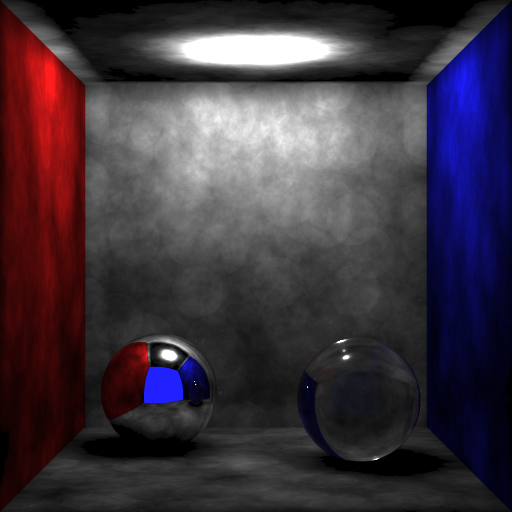
\includegraphics[width=\textwidth]{./images/renders/direct_photon_comp/photon_50000.png}
	\caption{25,000 photons}
	\end{subfigure}
	\begin{subfigure}[c]{0.3\textwidth}
	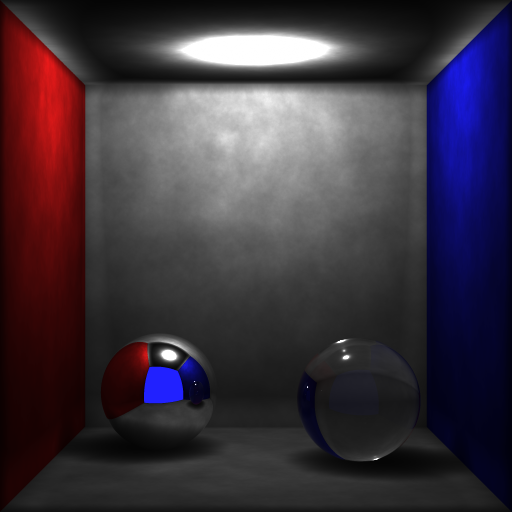
\includegraphics[width=\textwidth]{./images/renders/direct_photon_comp/photon.png}
	\caption{500,000 photons}
	\end{subfigure}
	\begin{subfigure}[c]{0.3\textwidth}
	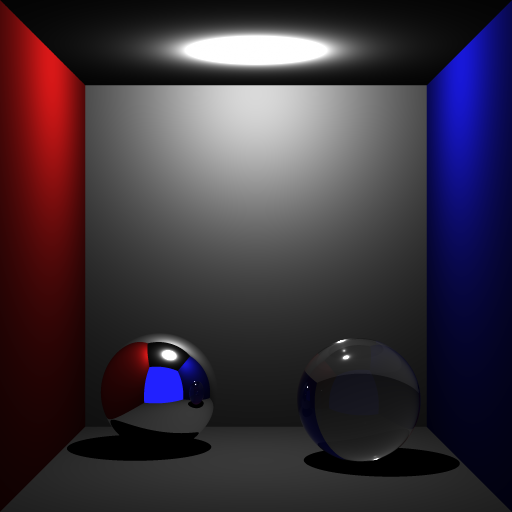
\includegraphics[width=\textwidth]{./images/renders/direct_photon_comp/direct.png}
	\caption{Raytraced}
	\end{subfigure}
	\caption{Comparison of the photon map radiance esitmate with direct illumination}
\label{fig:direct_compare}
\end{figure}

The system currently supports two types of light, point lights and area light, we will first consider calculating the radiance
from a point light as it is the simpler of the two cases.

The radiance from a point light is constant for all points at the same distance from the origin of the light, the radiance at
a point in the scene is given by Equation~\ref{fig:point_light_radiance}, where the function V is the visibility function, that
is if the point of intersection cannot see the point light it will not contribute the radinace at that point, this will cause
the appearance of shadows in the render.

In the case of area lights calculating the radiance at a point is more complicated, we must calculate the preportion of the
area of the light that is visible at the point of intersection, to do this we sample a number of shadow rays that evaluate the
visibility function across the area of the light.

\begin{figure}
	\centering
	\begin{subfigure}[c]{0.4\textwidth}
	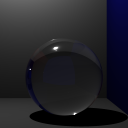
\includegraphics{./images/renders/refraction/render-schlick.png}
	\end{subfigure}
	\begin{subfigure}[b]{0.4\textwidth}
	\begin{equation}
	\centering
		E(x) = \frac
		{
			\Phi_s \cos{\theta}
		}
		{
			4 \pi r^2
		}
	\end{equation}
	\end{subfigure}
\end{figure}

\missingfigure{Area light figure}

\subsubsection{Texture Mapping}
Performing texture mapping requires the ability to query the texture coordinates at a point of intersection, for mesh objects this
will interpolate the barycentric coordinates for the triangle of intersection, spheres use a spherical mapping that uses the
spherical coordinates to generate u,v values, we use linear sampling to calculate the colour from the texture.

\subsection{Specular Reflection and Transmission}
\begin{equation*}
	\int_{\Omega}
	f_{r,S}(x, \omega, \omega')
	(
		L_{i,d}(x,\omega,\omega')
		+
		L_{i,c}(x,\omega,\omega')
	)
	(\omega \cdot n)d\omega'
\end{equation*}
For specular surfaces we again use raytracing to evaluate the contribution, as mentioned previousely the BRDF for specular surfaces
contains two delta functions (one for incoming ray and one for outgoing ray) as a result we cannot use the photon map to evaluate
the contribution from specular surfaces, we will again use raytracing to evaluate this component by tracing an additional reflected
or refracted ray, the equations used to calcualte these rays are given in Equations ~\ref{eq:reflections} and ~\ref{eq:refraction}

\begin{equation}
\cos{\theta_t} = \sqrt{1 - \left(\frac{\eta_1}{\eta_2}\sin{\theta_i}\right)^2}
\end{equation}

\todo{Add the reflection and refraction equations}
\subsubsection{Fresnel Reflection}
Transmissive surfaces reflect a proportion of the radiance incident at the surface as it passes from a material with a different
index of refraction, this proportion is determined by the fresnell equation for dielectrics, which is a function of the refractive
index of the two materials and the incident angle, this is given by equation ~\ref{eq:fresnel}

\begin{equation}
R_f(\theta)
=
\frac{
	\left(
	\frac
	{
	\eta_2 \cos{\theta_i} - \eta_1 \cos{\theta_t}
	}
	{
	\eta_2 \cos{\theta_i} + \eta_1 \cos{\theta_t}
	}
	+
	\frac
	{
	\eta_1 \cos{\theta_i} - \eta_2 \cos{\theta_t}
	}
	{
	\eta_1 \cos{\theta_i} + \eta_2 \cos{\theta_t}
	}
\right)^2
}{2}
\label{eq:fresnel}
\end{equation}

\subsubsection{Schlick Approximation}
Calculating the fresnel term for each refracted ray calculation can be costly, we can howerver use an approximation of the fresnel term
by Sclick this is given by:

\begin{equation}
R_s(\theta)=R_0 + \left(1 + R_0\right)\left(1 - \cos\theta\right)^5
\label{eq:schlick}
\end{equation}

where $R_0$ is the fresnel reflectance value for a ray parallel to the surface normal which can be precomputed,
this has been been shown to be up to 30\% faster than calculating the fresnel term for each refracted ray, Figure~\ref{fig:shlick-compare}
demonstrates the affect of accounting for the fresnell term and also using the Schlick approximation.

As with other aspects of the system where multiple rays can be spawned from a surface interaction (in this case one reflected and one refracted ray)
we use russian roulette in order to determine if we reflect or refract.

\begin{figure}[h]
\centering
\begin{subfigure}[b]{0.3\textwidth}
	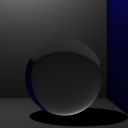
\includegraphics[width=\textwidth]{./images/renders/refraction/no-reflection.png}
	\caption{no fresnel reflection}
\end{subfigure}
\begin{subfigure}[b]{0.3\textwidth}
	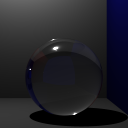
\includegraphics[width=\textwidth]{./images/renders/refraction/fresnel-reflection.png}
	\caption{true fresnel reflection}
\end{subfigure}
\begin{subfigure}[b]{0.3\textwidth}
	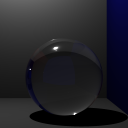
\includegraphics[width=\textwidth]{./images/renders/refraction/render-schlick.png}
	\caption{schlick fresnel reflection}
\end{subfigure}
\caption{Demonstration of Fresnell reflection and the Schlick approximation}
\label{fig:shlick-compare}
\end{figure}

\subsection{Diffuse Interreflection}
\begin{equation*}
		\int_{\Omega}
			f_{r,D}(x, \omega, \omega')
			L_{i,d}(x,\omega,\omega')
			(\omega \cdot n)d\omega'
\end{equation*}

Diffuse interrefection is the contribution that occurs from photons that have been bounced from a diffuse surface at least once
$(\mathbf{LD(S|D)^+E})$ while it is possible to estimate the contribition to the radiance at an intersection point directly from the photon map this
approach can cause visual artifacts due to variance in the estimate in order to reduce these artifacts we perfom a final gather
stage at the point of intersect that produces a diffuse ray that is traced into the scene until a non-specular object is intesected,
we then perform the radiance estimagte at this point and use this information to estimate the radiance incident at the original point of
intersection.  In order for the final gather to produce a correct estimate of the radiance we need to perform this stage multiple times per pixel,
as we are performing distributed raytracing this is a trivial addition.

\begin{figure}
\centering
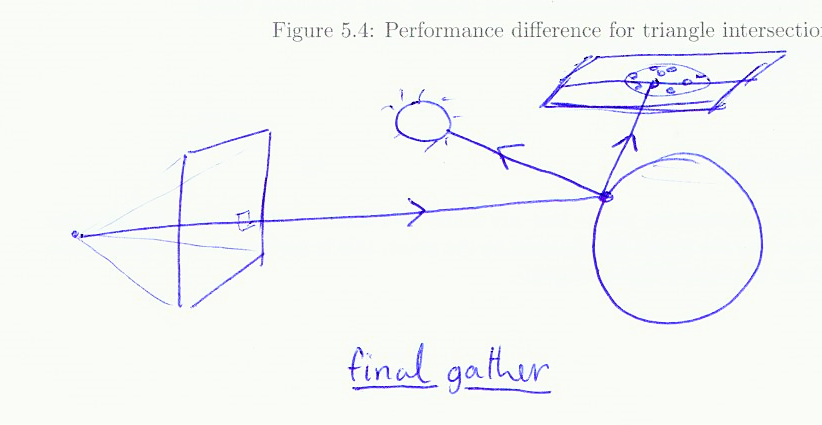
\includegraphics[width=\textwidth]{./images/final_gather.png}
\label{fig:final_gather}
\caption{Final Gather}
\end{figure}

\subsection{Caustics}
\begin{equation*}
		\int_{\Omega}
			f_{r,D}(x, \omega, \omega')
			L_{i,c}(x,\omega,\omega')
			(\omega \cdot n)d\omega'
\end{equation*}

Caustic light occures due to the focusing effect of curved specular surfaces, in other global illumination algorithms
caustics have been hard to simulate \cite{Jensen96a} and often cause large amounts of noise in the final image
with the photon map we are able to estimate the radiance directly from the caustic photon map, as we have seperated the
caustic photons from all other photon paths we reduce the nose that is introduced by caustics in all other radiance
estimates using the photon map. As caustics generally cause sharp visual effects using to few photons in the radiance
estimate can cause unwanted bluring \cite{JensenBook}, in order to reduce this we use a filter as part of the radiance estimate such
that photons near the query point contribute more to the radiance estimate, Jensen suggests the use of one of two filters, the
cone filter and the gaussian filter, each requiring a modification to the photon mapping radiance estimate.

\subsubsection{Cone Filter}
We use the cone filter by applying a weight $w_{pc}$ based upon the distance of the photon from the query point, this will
cause photons that are closer to the point to contribute more to the radiance estimation.

\begin{equation}
w_{pc} = 1 - \frac{d_p}{k r}
\end{equation}

where $k$ is the filter parameter, $d_p$ the distance of the photon from the query point and $r$ the maximum radius of
all photons found in the nearest neighbour search, the updated radiance estimate for the cone fileter is given by:

\begin{equation}
L_r(x, \vec{\omega}) \approx
\frac
{\sum\limits_{p=1}^N f_r(x, \vec{\omega}_p,\vec{\omega})\Delta \Phi_p(x,\vec{\omega}_p)w_{pc}}
{(1 - \frac{2}{3k})\pi r ^2}
\end{equation}

the term $(1 - \frac{2}{3k})$ is a normalisation factor for the cone filter \cite{Foley97}


\begin{figure}[h]

\centering
\begin{subfigure}[b]{0.4\textwidth}
	
\includegraphics[width=\textwidth]{./images/renders/no-filter.png}
	\caption{without the cone filter}
\end{subfigure}
\begin{subfigure}[b]{0.4\textwidth}
	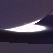
\includegraphics[width=\textwidth]{./images/renders/filter.png}
	\caption{with the cone filter}
\end{subfigure}
\caption{Comparison with and without cone filter}

\end{figure}

\newpage
\section{Participating Media}

In the case of a ray that intersects a participating media before intersecting a surface we need to calculate three components to
the radiance along the path of the ray in the medium, these are single scattering direct illumination, multiple scattering (in-scattering)
and attenuation (out-scattering)

\subsection{Ray Marching}
In order to evaluate the radiace from the participating media we perform a ray-march, this is an iterative operation that evaluates the
radiance along the ray as it moves through the participating media.

\begin{equation}
L(x, \omega) = \sum\limits_{i = 1}^N L_l(x, \omega_l')p(x, \omega_l', \omega)\sigma_s(x)\Delta x + e^{- \sigma_t \Delta x} L (x + \omega \Delta x, \omega)
\end{equation}

\subsection{Attenuation}
As a ray travels through a medium the radiance can be reduced due to out-scattering and absortion, this can be calculated by evaluating
the integral given in equation \todo{Add the equation}, as we are only considering homogeneous participating media this can be
simplified as the properties being integrated are constant and a closed form solution is possible.

\missingfigure{Attenuation Equation}

\subsection{Direct Illumination}
At each point in the ray march we also evaluate the contribution from each light in the scene due to single scattering, this is performed
by performing an additional ray march in the direction of the light and evalute the radiance arriving at the point on the ray.

\subsection{Muliple Scattering}
In order to evaluate the effect of multiple scattering within the participating media we use the photon map and the volume radiance estimate
for the photon map, as with direct illumination we evaluate the in-scattering at distctreate points along the path of the ray.

